%%%%%%%%%%%%%%%%%%%%%%%%%%%%%%%%%%%%%%%%%
% Programming/Coding Assignment
% LaTeX Template
%
% This template has been downloaded from:
% http://www.latextemplates.com
%
% Original author:
% Ted Pavlic (http://www.tedpavlic.com)
%
% Note:
% The \lipsum[#] commands throughout this template generate dummy text
% to fill the template out. These commands should all be removed when 
% writing assignment content.
%
% This template uses a Perl script as an example snippet of code, most other
% languages are also usable. Configure them in the "CODE INCLUSION 
% CONFIGURATION" section.
%
%%%%%%%%%%%%%%%%%%%%%%%%%%%%%%%%%%%%%%%%%

%----------------------------------------------------------------------------------------
%	PACKAGES AND OTHER DOCUMENT CONFIGURATIONS
%----------------------------------------------------------------------------------------

\documentclass[11pt,norsk,a4paper]{article}

\usepackage{ucs,babel}
\usepackage{fancyhdr} % Required for custom headers
\usepackage{lastpage} % Required to determine the last page for the footer
\usepackage{extramarks} % Required for headers and footers
\usepackage[usenames,dvipsnames]{color} % Required for custom colors
\usepackage{graphicx} % Required to insert images
\usepackage{listings} % Required for insertion of code
\usepackage{courier} % Required for the courier font
\usepackage{lipsum} % Used for inserting dummy 'Lorem ipsum' text into the template
\usepackage[utf8]{inputenc} %For "spesielle" tegn som æ, ø, å og andre er det anbefalt å angi dette. Mac brukere kan vurdere applemac og ikke utf8
\usepackage{amssymb}
\usepackage{framed, color}

\definecolor{shadecolor}{rgb}{0.9,0.9,0.9}



% Margins
\topmargin=-0.45in
\evensidemargin=0.75in
\oddsidemargin=0.75in
\textwidth=5in
\textheight=9.0in
\headsep=0.25in

\linespread{1.1} % Line spacing

% Set up the header and footer
\pagestyle{fancy}
\lhead{\hmwkAuthorName} % Top left header
\rhead{ \hmwkTitle} % Top center head
%\rhead{\firstxmark} % Top right header
\lfoot{\lastxmark} % Bottom left footer
\cfoot{} % Bottom center footer
\rfoot{Side\ \thepage\ av\ \protect\pageref{LastPage}} % Bottom right footer
\renewcommand\headrulewidth{0.4pt} % Size of the header rule
\renewcommand\footrulewidth{0.4pt} % Size of the footer rule

%\setlength\parindent{0pt} % Removes all indentation from paragraphs

\usepackage{empheq}
\usepackage[dvipsnames,table]{xcolor}
\definecolor{medGray}{RGB}{230,230,230}

\newenvironment{important}[2][]{
\setkeys{EmphEqEnv}{#2}
\setkeys{EmphEqOpt}{box={\setlength{\fboxsep}{10pt}\colorbox{medGray}},#1}
\EmphEqMainEnv}
{\endEmphEqMainEnv}

%----------------------------------------------------------------------------------------
%	CODE INCLUSION CONFIGURATION
%----------------------------------------------------------------------------------------

\definecolor{MyDarkGreen}{rgb}{0.0,0.4,0.0} % This is the color used for comments
\lstloadlanguages{Perl} % Load Perl syntax for listings, for a list of other languages supported see: ftp://ftp.tex.ac.uk/tex-archive/macros/latex/contrib/listings/listings.pdf
\lstset{language=Perl, % Use Perl in this example
        frame=single, % Single frame around code
        basicstyle=\small\ttfamily, % Use small true type font
        keywordstyle=[1]\color{Blue}\bf, % Perl functions bold and blue
        keywordstyle=[2]\color{Purple}, % Perl function arguments purple
        keywordstyle=[3]\color{Blue}\underbar, % Custom functions underlined and blue
        identifierstyle=, % Nothing special about identifiers                                         
        commentstyle=\usefont{T1}{pcr}{m}{sl}\color{MyDarkGreen}\small, % Comments small dark green courier font
        stringstyle=\color{Purple}, % Strings are purple
        showstringspaces=false, % Don't put marks in string spaces
        tabsize=5, % 5 spaces per tab
        %
        % Put standard Perl functions not included in the default language here
        morekeywords={rand},
        %
        % Put Perl function parameters here
        morekeywords=[2]{on, off, interp},
        %
        % Put user defined functions here
        morekeywords=[3]{test},
       	%
        morecomment=[l][\color{Blue}]{...}, % Line continuation (...) like blue comment
        numbers=left, % Line numbers on left
        firstnumber=1, % Line numbers start with line 1
        numberstyle=\tiny\color{Blue}, % Line numbers are blue and small
        stepnumber=5 % Line numbers go in steps of 5
        }

% Creates a new command to include a perl script, the first parameter is the filename of the script (without .pl), the second parameter is the caption
\newcommand{\perlscript}[2]{
\begin{itemize}
\item[]\lstinputlisting[caption=#2,label=#1]{#1.pl}
\end{itemize}
}

%----------------------------------------------------------------------------------------
%	DOCUMENT STRUCTURE COMMANDS
%	Skip this unless you know what you're doing
%----------------------------------------------------------------------------------------

% Header and footer for when a page split occurs within a problem environment
\newcommand{\enterProblemHeader}[1]{
\nobreak\extramarks{#1}{#1 continued on next page\ldots}\nobreak
\nobreak\extramarks{#1 (continued)}{#1 continued on next page\ldots}\nobreak
}

% Header and footer for when a page split occurs between problem environments
\newcommand{\exitProblemHeader}[1]{
\nobreak\extramarks{#1 (continued)}{#1 continued on next page\ldots}\nobreak
\nobreak\extramarks{#1}{}\nobreak
}

\setcounter{secnumdepth}{0} % Removes default section numbers
\newcounter{homeworkProblemCounter} % Creates a counter to keep track of the number of problems

\newcommand{\homeworkProblemName}{}
\newenvironment{homeworkProblem}[1][Problem \arabic{homeworkProblemCounter}]{ % Makes a new environment called homeworkProblem which takes 1 argument (custom name) but the default is "Problem #"
\stepcounter{homeworkProblemCounter} % Increase counter for number of problems
\renewcommand{\homeworkProblemName}{#1} % Assign \homeworkProblemName the name of the problem
\section{\homeworkProblemName} % Make a section in the document with the custom problem count
\enterProblemHeader{\homeworkProblemName} % Header and footer within the environment
}{
\exitProblemHeader{\homeworkProblemName} % Header and footer after the environment
}

\newcommand{\problemAnswer}[1]{ % Defines the problem answer command with the content as the only argument
\noindent\framebox[\columnwidth][c]{\begin{minipage}{0.98\columnwidth}#1\end{minipage}} % Makes the box around the problem answer and puts the content inside
}

\newcommand{\homeworkSectionName}{}
\newenvironment{homeworkSection}[1]{ % New environment for sections within homework problems, takes 1 argument - the name of the section
\renewcommand{\homeworkSectionName}{#1} % Assign \homeworkSectionName to the name of the section from the environment argument
\subsection{\homeworkSectionName} % Make a subsection with the custom name of the subsection
\enterProblemHeader{\homeworkProblemName\ [\homeworkSectionName]} % Header and footer within the environment
}{
\enterProblemHeader{\homeworkProblemName} % Header and footer after the environment
}

%----------------------------------------------------------------------------------------
%	NAME AND CLASS SECTION
%----------------------------------------------------------------------------------------

\newcommand{\hmwkTitle}{Øving\ \#6} % Assignment title
\newcommand{\hmwkDueDate}{Mandag,\ 15\ April,\ 2013} % Due date
\newcommand{\hmwkClass}{TMA4280\ } % Course/class
\newcommand{\hmwkClassTime}{} % Class/lecture time
\newcommand{\hmwkClassInstructor}{} % Teacher/lecturer
\newcommand{\hmwkAuthorName}{Simen Haugerud Granlund \&\ Steffen Pøhner Henriksen} % Your name

%----------------------------------------------------------------------------------------
%	TITLE PAGE
%----------------------------------------------------------------------------------------

\title{
\vspace{2in}
\textmd{\textbf{\hmwkClass:\ \hmwkTitle}}\\
\normalsize\vspace{0.1in}\small{Innleveringsdato\ \hmwkDueDate}\\
\vspace{0.1in}\large{\textit{\hmwkClassInstructor\ \hmwkClassTime}}
\vspace{3in}
}

\author{\textbf{\hmwkAuthorName}}
\date{} % Insert date here if you want it to appear below your name

%----------------------------------------------------------------------------------------

\begin{document}

\maketitle

%----------------------------------------------------------------------------------------
%	TABLE OF CONTENTS
%----------------------------------------------------------------------------------------

%\setcounter{tocdepth}{1} % Uncomment this line if you don't want subsections listed in the ToC

\newpage
 \tableofcontents
\newpage

%----------------------------------------------------------------------------------------
%	SOLUTION
%----------------------------------------------------------------------------------------

% To have just one problem per page, simply put a \clearpage after each problem
\section{Diskretisering av Poissons ligning}

Programmet skal kunne løse Poisson-ligningen i domenet $ x= [0..1], y = [0..1]. $ Poisson-ligningen er på formen:

\begin{equation} 
-\Delta^2\phi = f(x,y)
\end{equation}
\begin{equation}
-\Delta^2\phi = -\frac{\partial^2\phi}{\partial x^2} - \frac{\partial^2\phi}{\partial x^2} = -u_{xx}-u_{yy} = f(x,y)
\end{equation}

Vi trenger en form av denne som kan løses numerisk. Den må diskretiseres slik at en datamaskin skal kunne løse den. For å få til dette forsøker vi å Taylor-utvikle i  x-, og y-retning. Viser kun utviklingen i x-retning da utregningene er tilsvarende for y.

\begin{equation}
u(x+h,y) = u(x,y) + hu_x(x,y) + \frac{1}{2}h^2u_{xx}(x,y) + \frac{1}{6}h^3u_{xxx}(x,y)+ ...
\end{equation}
\begin{equation}
u(x-h,y) = u(x,y) - hu_x(x,y) + \frac{1}{2}h^2u_{xx}(x,y)- \frac{1}{6}h^3u_{xxx}(x,y)+ ...
\end{equation}

Vi ser bortifra høyere ordens ledd ($h^3, h^4$...), og løser for $u_{xx}$.

\begin{equation}
u_{xx}(x,y) \approx \frac{1}{h^2}(u(x+h,y)-2u(x,y)+u(x-h,y))
\end{equation}

Dermed har vi nå et uttrykk for $u_{xx}$ som er lettere å forstå for en datamaskin. Tilsvarende har vi et uttrykk for $u_{yy}$. Vi legger disse sammen og får et diskretisert uttrykk for Poisson-ligningen, også kalt fem-punktsformelen.

\begin{important}{equation}
-u(x+h,y)-u(x,y+h)-u(x-h,y)-u(x,y-h)+4u(x,y) = h^2f(x,y)
\end{important}

I (6) betegner $f$ hvor finkjemmet rutenett som benyttes (steglengden). Det diskretiserte uttrykket løser problemet i punkt for punkt, og tettheten til punktskyen avhenger av h. Vi kan se at hvert punkt avhenger av nabopunktene (firer-naboer) i x- og y-retning både negativt og positivt. Utifra den observasjonen kan vi sette opp et stensil som gjør det enklere å se hva den betyr.

\begin{figure}[h]
\centering
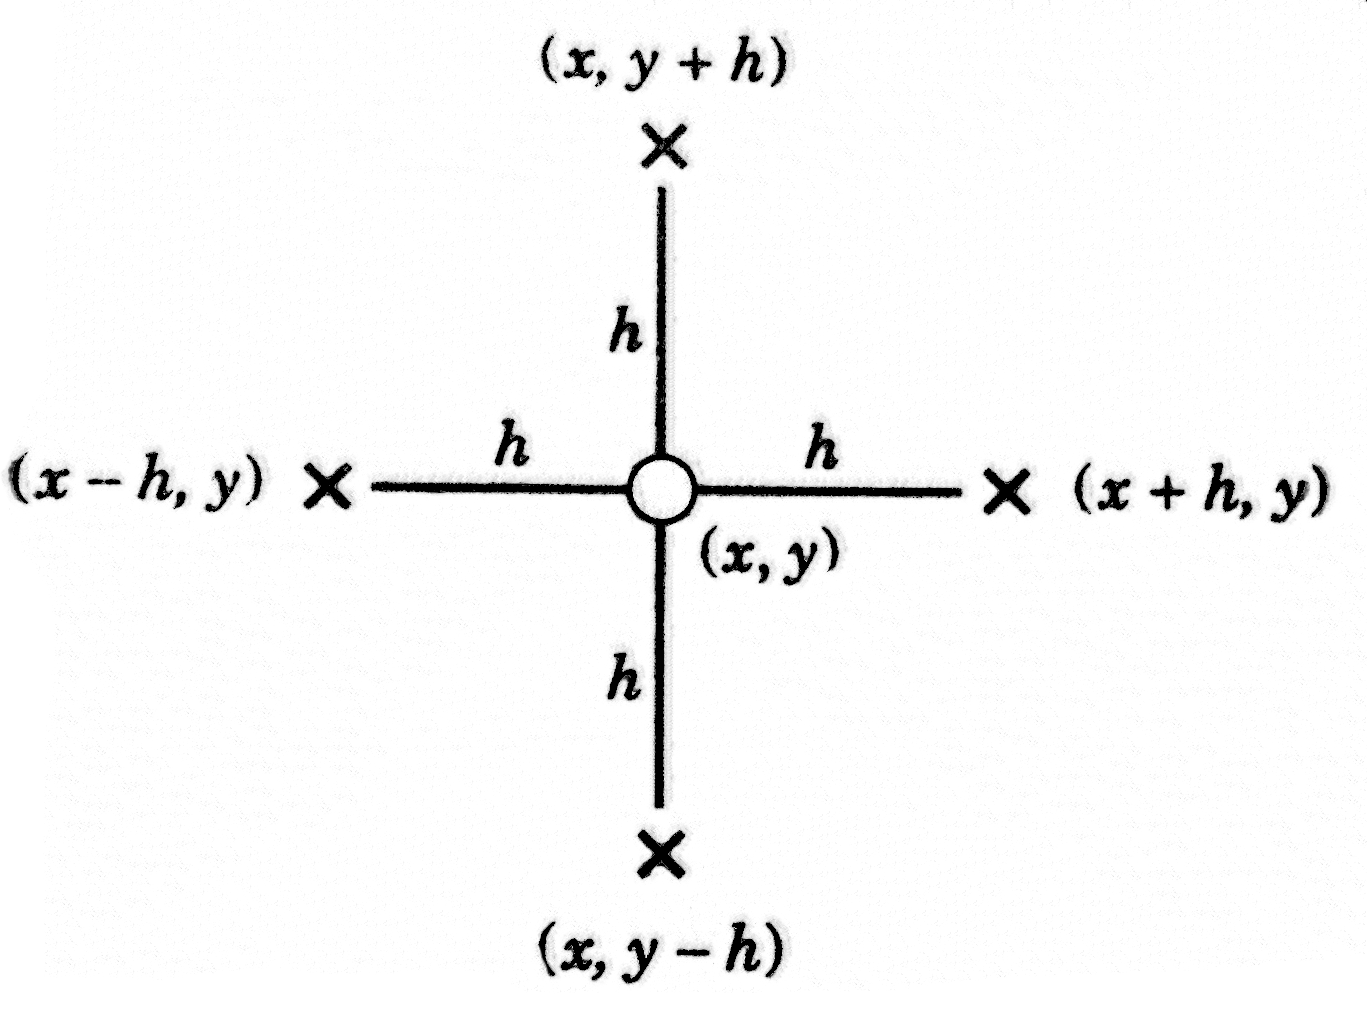
\includegraphics[scale=0.2]{five.png}
\caption{Fem-punkts stensil \cite{ky}}
\end{figure}

Utifra stensilen kan vi sette opp en ligning for hvert punkt. Høyresiden blir $h^2f(x,y)$ hvor x og y betegner posisjonen til punktet vi ser på i domenet. Venstresiden refererer til hvert nabopunkt en gang, og til seg selv 4 ganger. Om et refererende punkt ligger på grensen til domenet ersattes dette med grensebetingelsen, f.eks 0 ved Dirichlet-betingelser.

Vi kan sette ligningene sammen til et system på formen \textbf{Ax = b}. Som kan løses av en datamaskin på mange måter. Antall punkt, og dermed antall ligninger, avhenger av $h$, og vokser i graden $h^2$. Det betyr at dersom vi halverer steglengden $h$, firedobler vi antall ligninger maskinen må løse. 

\section{Løsning av ligningssystemet}

For å løse Poissons ligning gjenstår å løse ligningssystemet $AU=B$. Dimensjonen på matrisen A er $(N-1)^2$, og er 'sparse'. Matrisen er en båndmatrise med båndbredde lik $b=n$. Et slikt ligningssystem kan løses ved mange ulike metoder, og er et viktig tema innen numerisk algebra og algoritmer. Oppgaven krever at vi løser systemet ved bruk av FST (Fast Sine Transform). FST er implementert i en gitt Fortran-kode som vi skal anse som en 'black box'. Koden utfører en diskret sinustransformasjon og dets inverse motpart.

\subsection{Diagonalisering}

Gitt systemet:

$$ AU=B $$

Deretter kan vi konvertere B til eigenvectorrommet ved hjelp av S som her er sinus transformasjonen gitt slik:

$$ \widetilde{B} = S^{-1}((S(B))^T) $$

Med dette kan vi finne $\widetilde{U}$ ved å skalere med eigenverdier

$$ \widetilde{u}_{i,j} = \frac{\widetilde{b}_{i,j}}{\lambda_{i}+\lambda_{j}} \quad 1 \leq i,1 \leq n-1 $$

Ved hjelp av uttrykket for $\widetilde{U}$ kan vi finne løsningen $U$

$$ U = S^{-1}((S(\widetilde{U}^T))^T) $$

\subsection{Verifikasjon av resultat}

Vi må verifisere at programmet vårt gjør beregningene riktig. Dette gjør vi ved å benytte en verdi for $f(x,y)$ som vi vet fører til en kjent analytisk løsning $u(x,y)$. Ved å sammenligne den eksakte løsningen $u(x,y)$ med løsningen programmet vårt gir kan vi finne den maksimale punktfeilen. Det er forventet at punktfeilen reduseres når vi øker antall beregningspunkter. 

$$ -\Delta u = f(x,y) = 5\pi^2sin(\pi x)sin(2\pi y) $$

som gir den analytiske løsningen

$$ u(x,y) = sin(\pi x)sin(2\pi y) $$

Programmet returnerer den maksimale punktvise feilen. Om denne er tilstrekkelig liten konkluderer vi med at resultatet er korrekt. 


\section{Programmet}

\subsection{Parallellprosessering}

\subsubsection{MPI}
For å kunne kjøre programmet på flere prosessorer er det nødvendig å dele opp problemet i mindre deler. MPI-biblioteket\cite{MPI} gjør oss i stand til å kjøre programmet over flere uavhengige prosesser. Ved å dele matrisen B i kolonner og fordele disse utover MPI-prosessene kan vi gjøre sinustransformasjoner parallelt. Dette innfører en ny utfordring da hver prosess har informasjon som trengs av andre prosesser ved transponeringen av matrisen B. Vi må sende data over nettverk for å kunne transponere matrisen. For å gjøre dette deler vi opp kolonnene inn i blokker hvor hver blokk skal sendes til en annen prosess. Det er MPI-kallet MPI\_Alltoallv som sender dataene. Dette kallet kan sende en vektor og informasjon om hvilken prosess som trenger hvilken del av denne vektoren. Derfor transformeres kolonnene til en lang vektor sortert etter blokkoppdelingen. Når de respektive vektorer blir mottatt av den prosessen de hører til blir disse så transformert tilbake til en matrise for videre beregninger. Tilbaketransformasjonen sørger for at matrisen nå er transponert.

\begin{figure}[h]
\centering
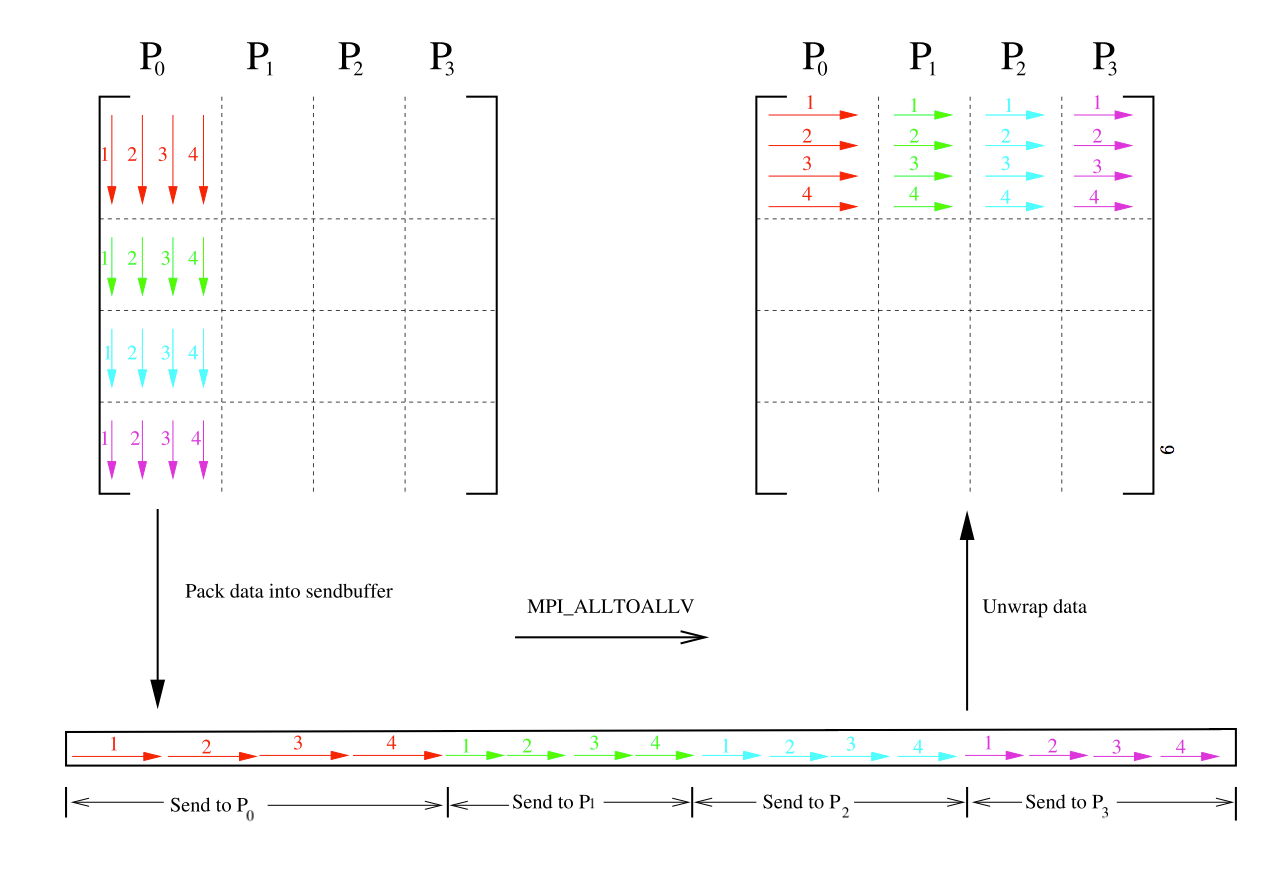
\includegraphics[scale=0.3]{transpose.png}
\caption{Figur hentet fra oppgaveteksten om transponeringen}
\end{figure}

Når beregningene er ferdige er resultatene spredd utover prosessene. Resultatet er den maksimale punktvise feilen i forhold til den eksakte løsningen. Vi er interessert i den maksimale punktvise feilen over alle prosesser og ikke på hver enkelt prosess. Vi finner den maksimale globale feilen ved å bruke MPI-funksjonen MPI\_Reduce med opsjonen MPI\_MAX. På denne måten får vi et resultat og ikke et for hver prosess.

I tillegg har vi laget en funksjon som samler inn verdien i hvert beregningspunkt fra alle prosesser og kombinerer dette i én matrise. Denne matrisen kan vi så bruke for å visualisere resultatet med for eksempel Gnuplot\cite{gnuplot}. Dette gjøres med funksjonen MPI\_Gatherv. For å kunne sende dataene ved hjelp av denne funksjonen må vi på samme måte som ved bruken av MPI\_Alltoallv transformere prosessenes matriser til en vektor. Deretter kan vi pakke ut vektoren på rotprosessen til løsningsmatrisa.

\begin{figure}[h]
\centering
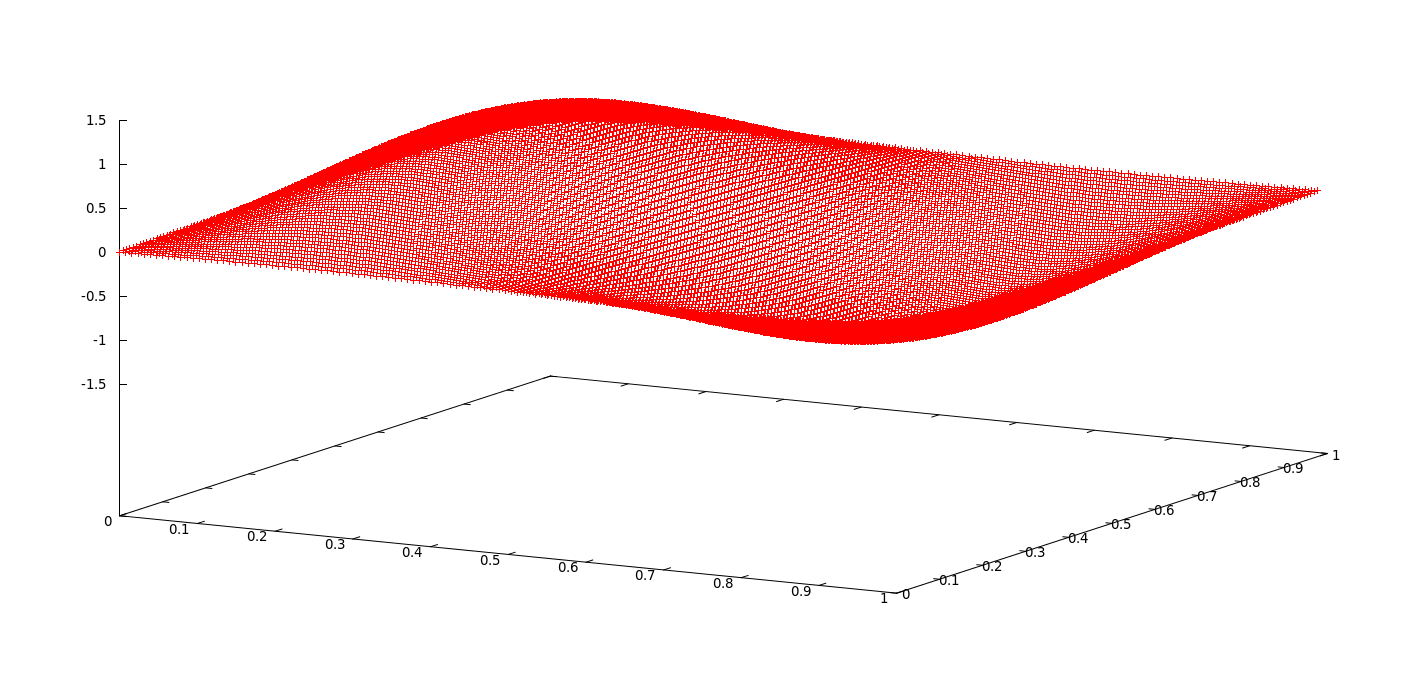
\includegraphics[scale=0.25]{plot_n128.png}
\caption{Visualisering av løsningen ved 16384 beregningspunkter (n=128). $f(x,y)=5\pi^2sin(\pi x)sin(2\pi y)$}
\end{figure}

\subsubsection{OpenMP}
Videre kan ytterligere forbedringer gjøres for å forbedre parallelliteten. Ved å bruke OpenMP\cite{MP} kan vi bruke flere tråder innen hver prosess slik at sinustransformasjonen gjennomføres ved en høyere grad av parallellitet. Her dukker det opp en utfordring med minnebruk da hver tråd krever en del av minne for å kunne utføre sinustransformasjonen. FORTRAN-koden krever en arbeidsbuffer. For å kunne benytte OpenMP må hver tråd ha sin egen uavhenige buffer. Om vi hadde brukt samme buffer kunne tråder ha lest og skrevet til samme sted i minne. Dette unngår vi ved å samle arbeidsbufferene i en matrise som kolonner. Antall kolonner er lik antall tilgjenglige tråder satt av en miljøvariabelen. I parallell-seksjonen av for-løkka brukes metoden get\_thread\_num() for å gi tråden sitt uavhengige buffer. På denne måten blir fst-rutinen parallellisert ytterligere. Denne rutinen krever mange flyttallsoperasjoner, og det er derfor lurt å bruke OpenMP her. Dog bruker vi mer minne ved å parallellisere fst-rutinen på denne måten.

Vi har valgt å ikke bruke OpenMP på de resterende for-loopene i koden selvom de er uavhengige og sådan kan parallelliseres. Dette er fordi de inneholder få flyttallsoperasjoner og overhead med join/forks gjort forbedringene nært neglisjerbart. 

\section{Kompilering}
Programmet ble kompilert C og FORTRAN-kompilator fra Intel. Vi brukte Intel versjon 11.1.059 og OpenMPI-bibliotek (versjon 1.4.3). CMAKE ble brukt til å lage et byggesystem for programmet. Da vi kjørte cmake brukte vi flagget -DCMAKE\_BUILD\_TYPE=Release for å skru på optimaliseringer i kompilatoren. Git\cite{git} ble brukt for å vedlikeholde kode på serveren og lokalt.

\section{Resultater}
Resultatene i denne rapporten ble til ved kjøring av programmet på \texttt{kongull} clusteren\cite{kongull}. Maksimalt tok vi i bruk tre noder med tilsammen 36 fysiske prosessorkjerner fordelt på 6 prosessorer og 2GB minne per node.

\begin{shaded}
\textbf{Kongull Cluster}\\
\begin{itemize}
\item{CentOS 5.3}
\item{93 beregningsnoder}
\item{2 AMD Opteron 2431 Istanbul 6-kjerner 2.4 GHz per noder}
\item{24 GB minne per node (48 GB for de priviligerte)}
\end{itemize}
\end{shaded}

\subsection{Speedup og parallellitet}
Det sekvensielle programmet vi sammenligner med er gitt med oppgaven. Hadde vi kjørt vårt program med en tråd og sammenlignet med dette hadde vi overestimert parallelliseringen av koden. Dette er fordi tiden eksekveringen tar for en parallellskrevet kode med en tråd som regel er lengre enn med en ren sekvensiell kode. 

Speedup $S_p$ er et mål på hvor mye raskere den parallelle koden er i forhold til den sekvensielle. 

$$ S_p = \frac{T_1}{T_p}$$
hvor $T_1$ er tiden det tar å kjøre programmet sekvensielt, $T_p$ er tiden det tar å kjøre programmet parallellt på $p$ prosessorer. 

\begin{figure}[h]
\centering
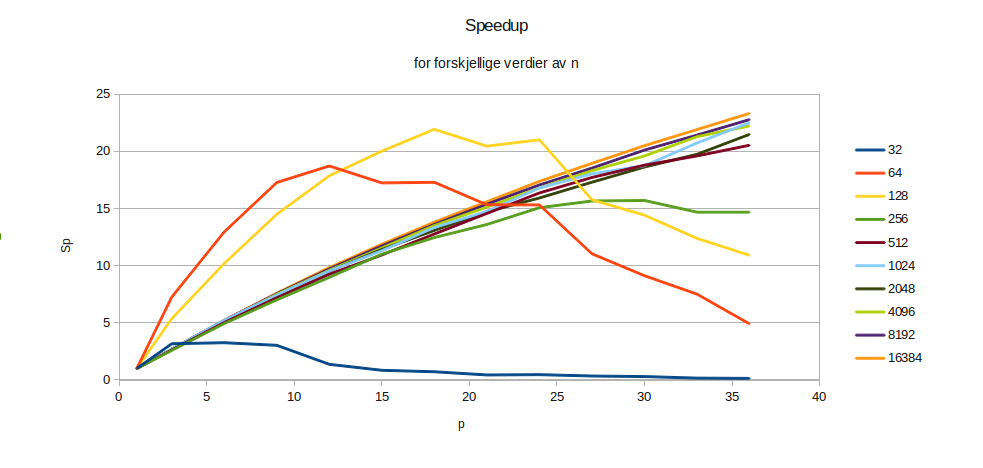
\includegraphics[scale=0.425]{plot_speedup.png}
\caption{Visualisering av speedup ved ulike p og n}
\end{figure}

Vi har også estimert den parallelle effektiviteten. Denne viser forholdet mellom speedup og antall prosessorer. 
$$ \eta_p = \frac{S_p}{p}$$

\begin{figure}[h]
\centering
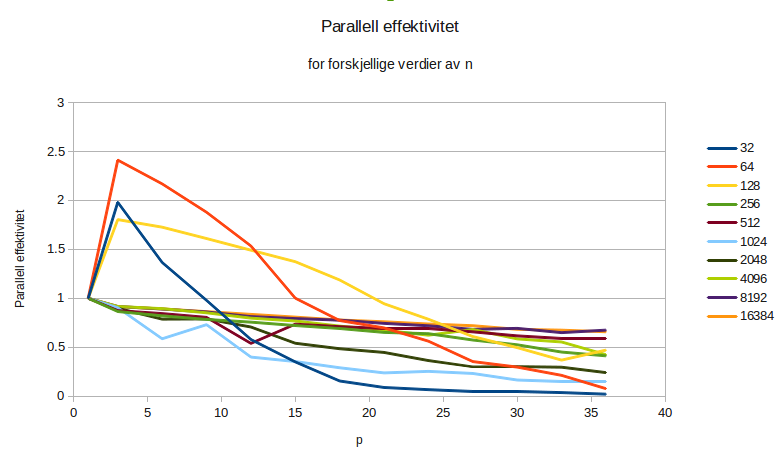
\includegraphics[scale=0.5]{plot_parallell.png}
\caption{Visualisering av parallell effektivitet $\eta_p$}
\end{figure}

\subsection{Tidsbruk}

Om vi tegner tidsbruken mot problemstørrelsen $n^2$ ser vi at tiden vi bruker på å løse systemet øker linært. 

\begin{figure}[h]
\centering
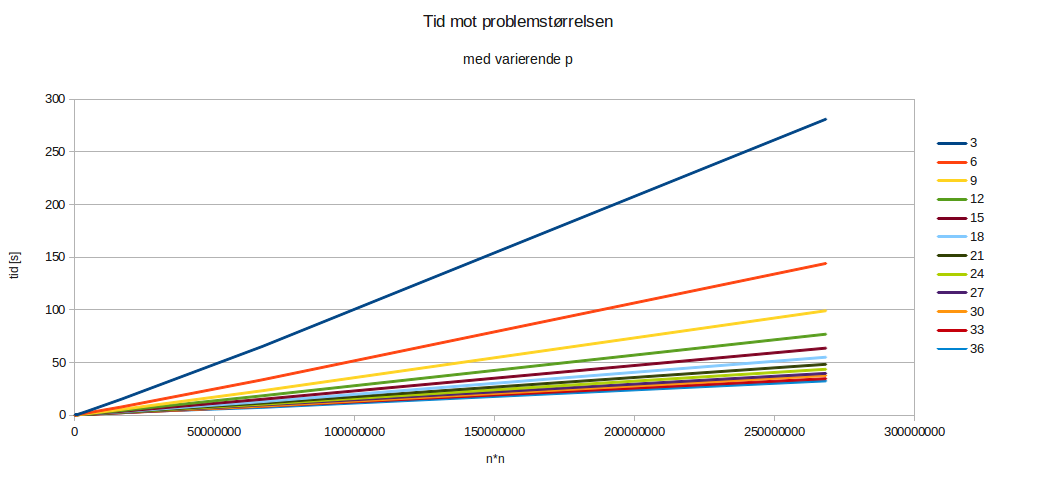
\includegraphics[scale=0.4]{plot_tid_p.png}
\caption{Visualisering tidsbruk mot problemstørrelsen}
\end{figure}



\subsection{Konvergenstest}
%TODO: Minker feilen med faktor fire når vi halverer steglengden?
Når vi øker antall beregningspunkter vil den maksimale punktfeilen, altså differansen mellom eksakt og beregnet løsning, minke. Vi har gjort en konvergenstest hvor vi tegner den maksimale punktfeilen mot problemstørrelsen og vi ser at punktfeilen minker raskt.

\begin{figure}[h]
\centering
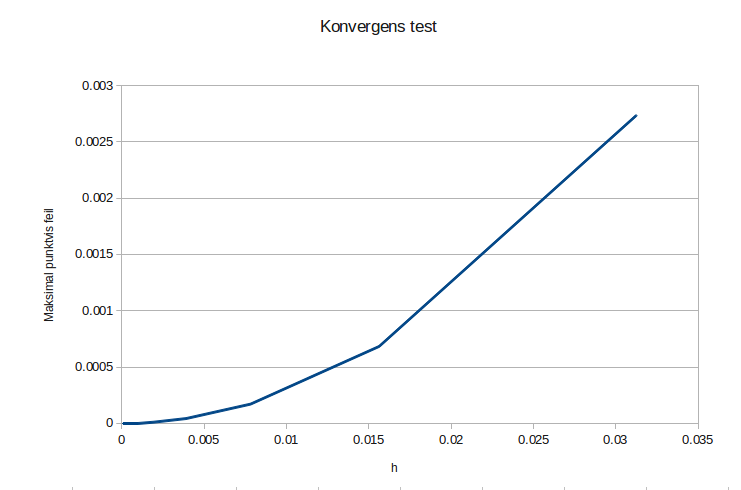
\includegraphics[scale=0.5]{plot_konvergens.png}
\caption{Logaritmisk graf som viser maksimal punktvis feil over problemstørrelse}
\end{figure}


\section{Analyse}

\subsection{Hybrid mot et rent MPI-program}

Gitt at $p*t=36$ hvor $p$ er antall MPI-prosesser og $t$ antall tråder per prosess ser vi at et rent MPI-program kjører raskere enn en hybrid-versjon. Dette tror vi er fordi en ren MPI-versjon vil parallellisere en større del av koden enn OpenMP. I MPI deler vi opp matrisen i striper hvor hver prosess får sin stripe. Dersom vi ofrer en MPI-prosess mot en tråd ekstra vil OpenMP tråden kun parallellisere fst-rutinen. Det virker som om nettverksforsinkelsen ved bruk av MPI ikke dominerer tidsbruken. Men dersom man har tilgang til flere tråder og ikke fler MPI-prosesser (for eksempel Intels Hyper Threading) vil hybridversjonen dra nytte av dette. 

\begin{figure}[h]
\centering
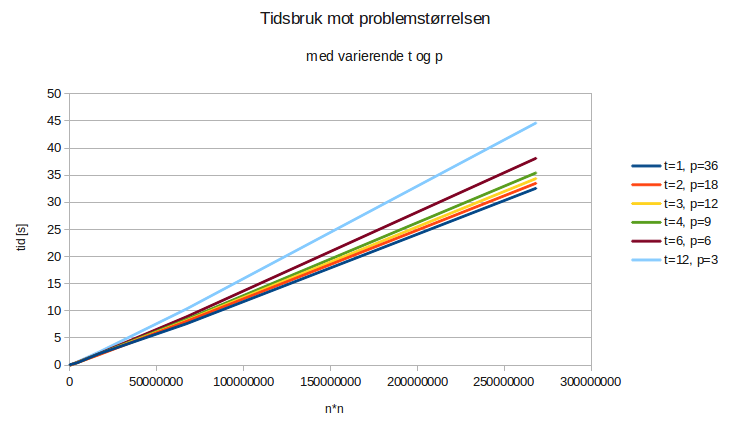
\includegraphics[scale=0.5]{plot_t_p.png}
\caption{Sammenheng mellom ulike verdier for t og p}
\end{figure}

\subsection{Speedup}

Vi ser at tiden det tar å løse problemet for et fast antall prosessorer øker linært med $n^2$. Dette er forventet. Øker vi $n$ med to firedobler vi problemstørrelsen og arbeidet for å løse problemet. Problemstørrelsen ($n^2$) og tiden det tar følger hverandre linært.

Vi ser at vi får en økning av speedup $S_p$ til vi når et metningspunkt og speedupen avtar. Dette er fordi problemstørrelsen i forhold til antall prosessorer er så liten at det ikke er fordelaktig å dele opp problemet ytterligere. Vi ser denne tendensen godt ved mindre problemstørrelser, men ved bruk av 36 prosessorer når vi ikke denne metningen ved problemstørrelser over $n=128$. Det er dog noen merkelige resultater å se. For eksempel oppnår vi en veldig dårlig speedup ved $n=1024$, men veldig god speedup på $n=512$. Dette klarer vi ikke helt å forklare. Det kan være at disse merklighetene er spesielle for denne kjøringen, og at vi hadde fått bedre resultater ved et større statistisk grunnlag.

\subsection{Endring av programmet for andre verdier for f}
Slik som vi har skrevet programmet er det enkelt å endre det til å løse et annet Poisson-problem. Funksjonen funcf returnerer verdien av f gitt en verdi for x og y. Skal vi bruke en annen funksjon er det kun en linje i denne funksjonen som må skrives om, og eventuelle konvergenstester.

Om vi skal la $f=0$ i hele domenet, men 1 i to punkt(som foreslått i oppgaven) kan vi lett endre funcf til å ta hensyn til dette. En if-spørring finner punktet hvor $f=1$ og gir dette tilbake.

\subsection{Ikke-homogene Dirichlet-grensebetingelser}
% Slik som programmet fremstår nå løser det Poisson-problem hvor vi vet at punktene på randen har verdien 0. Om dette ikke er tilfellet og vi har en ikke-homogen Diricihlet-grensebetingelse eller en annen verdi for randen må programmet modifiseres noe. Ligningssystemet som fempunktsstensilen gir er på formen $Ax=b$. Her må x- og b-vektorene utvides til å medregne randpunktene. Da vi vet verdien til grensepunktet settes denne i x-vektoren. I A-matrisen settes diagonalen til de kjente punktene lik 1 og resten av raden lik null. På denne måten tar nå programmet hensyn til ikke-homogene Dirichlet-grensebetingelser eller andre verdier på randen. Dette er ikke blitt implementert.
Slik som programmet fremstår nå løser det Poisson-problem hvor vi vet at punktene på randen har verdien 0. Om dette ikke er tilfellet og vi har en ikke-homogen Diricihlet-grensebetingelse eller en annen verdi for randen må programmet modifiseres noe. For å inkludere randpunktene i ligningssytemet innfører vi ny vektor på høyresiden av ligningen $Ax=b$ slik at vi får et system $Ax=b+c$. $c$ inneholder verdien til randpunktene og null der randpunktene ikke inngår i fempunktsstensilen. 

\subsection{Rektangulært domene}
Dersom vi skal løse Poisson-problemet på et rektangulært domene blir utgangspunktet forandret. Vi antar lik steglengde $h$ i begge retninger. Gitt domenet $\Omega = (0,L_x)*(0,L_y)$ får vi verdier for beregningspunktene slik

$$ x_i = ih, \quad i=0,1,...,n, \quad n = \frac{L_x}{h}  $$
$$ y_j = jh, \quad j=0,1,...,m, \quad m = \frac{L_y}{h} $$ 

$$
-u(i+h,j)-u(i,j+h)-u(i-h,j)-u(i,j-h)+4u(i,j) = h^2f(i,j) $$
$$\quad i=1,...,n-1 \quad j=1,...,m-1$$

Dette vil gi oss et system på formen $Ax=b$ som kan løses av programmet vårt med små modifikasjoner. Modifikasjonene innebærer å innføre $n$ og $m$. Og splitte matrisen med hensyn på de nye variablene.

\section{Konklusjon}

Vi har løst poissonproblem ved bruk av en FFT basert løser parallellt, ved bruk av MPI og OpenMP. I forhold til den sekvensielle løseren gitt med oppgaven løser vårt program store problemsett mye raskere. Vi har en speedup på opptil 24 ved bruk av 36 prosessorer. Forskjeller mellom MPI og OpenMP har blitt belyst. Våre resultater har vært i samsvar med teorien, men vi ser noen enkelttilfeller vi ikke kan forklare.


% EXAMPLE OF CODE INCLUSION: \lstinputlisting[language=C, firstline=53, lastline=71, caption=MPI version]{../src/oving4-openmpi.c}

%----------------------------------------------------------------------------------------

\begin{thebibliography}{99}

\bibitem{ky}
Erwin Kreyzig,
\emph{Advanced Engineering Mathematics}.
9th Edition,
2006.

\bibitem{MPI}
OpenMPI, Open Source High Performance Computing, \it{http://www.open-mpi.org/}, 12.04.2013

\bibitem{MP}
OpenMP, \it{http://www.open-mpi.org/}, 12.04.2013

\bibitem{gnuplot}
Gnuplot, \it{http://www.gnuplot.info/}

\bibitem{kongull}
Kongull hardware specs, \it{http://docs.notur.no/Members/hrn/kongull.hpc.ntnu.no/kongull-hardware-1/hardware}, 13.04.2013

\bibitem{git}
Git, \it{http://git-scm.com/}

\end{thebibliography}

%\listoftables
\listoffigures

\end{document}